\chapter{Likelihoods and cosmological parameters}

Bayes theorem\index{Bayes theorem}

\begin{figure}
  \begin{center}
    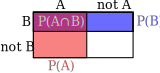
\includegraphics[width=0.7\textwidth]{figs/cosmological_parameters/bayes_theorem.pdf}
  \end{center}
  \caption{Diagram for Bayes theorem.  The probability for event A is in red and the probability for event B is in blue.  These overlap to form purple in the region of the probability of both events occuring jointly.}
\end{figure}


\begin{equation}
  P(A|B) = \frac{P(A\cap B)}{P(B)}
\end{equation}
      
\begin{equation}
  P(A|B) P(B) = P(A \cap B) =   P(B|A) P(A)
\end{equation}


posterior probability
likelihood
prior probability


\subsection{Gaussian likelihood in the case of supernovae}




\subsection{Markov Chain Monte Carlo}

\subsubsection{Detailed Balance}

\subsubsection{Metropolis-Hastings algorithm}

\subsubsection{Affine invariant algorithm}
emcee \citep{2013PASP..125..306F}

